\documentclass[12pt]{article}

% Packages
\usepackage{titlesec}
\usepackage{graphicx}
\usepackage{subcaption}
\usepackage{amsmath}
\usepackage{amsfonts}
\usepackage{amssymb}
\usepackage{hyperref}
\usepackage{enumitem}
\usepackage{times}
%\usepackage[nomarkers,figuresonly]{endfloat}


% Page layout
\usepackage[top=1in, bottom=1in, left=1in, right=1in]{geometry}

%% Title formatting
%\titleformat{\section}{\normalfont\Large\bfseries}{\thesection}{1em}{}
%\titleformat{\subsection}{\normalfont\large\bfseries}{\thesubsection}{1em}{}
%\titleformat{\subsubsection}{\normalfont\normalsize\bfseries}{\thesubsubsection}{1em}{}

% Title, author, date
\title{Report-Challenge 1}
\author{Da Vinchie Lisa, Pettenà Piero}
\date{\today} % or specify a specific date

\begin{document}
	
	\maketitle
	
	% Abstract if needed
	% \begin{abstract}
		% Your abstract goes here.
		% \end{abstract}
	
	% Table of Contents
	% \tableofcontents
	
	% Start of the content
	\section*{Introduction}
	In this challenge, our goal is to find an effective method to classify the images of the \textit{FashionMNIST} dataset, based on their content. The dataset is formed by black-and-white images of 28 $\times$ 28 pixel, each one representing a clothing item belonging to one of the following 10 categories: \textit{T-shirt or top}, \textit{Trouser}, \textit{Pullover}, \textit{Dress}, \textit{Coat}, \textit{Sandal}, \textit{Shirt}, \textit{Sneaker}, \textit{Bag} and \textit{Ankle boot}.
	
	\section*{Exercise 1}
	The goal of this exercise is to perform Principal Component Analysis (PCA) in order to find out how the clusters are separated. In order to do that, we performed two kinds of PCA: linear and kernel PCA; then, we plotted the first two and three principal components, coloring each data point with the original labels. In both cases, we used only 10000 randomly selected images, out of the 70000 images composing the \textit{FashionMNIST} dataset.\newline
	We started by using a linear PCA, obtaining the clustering in Figure \ref{fig:pca_linear}; although the data points appear to be grouped in clusters, it is clear how they are not well separated: some clusters have data points that are very far from their centroid, while others overlap.\newline
	Performing Kernel PCA with a Radial Basis Function kernel, using the default value of the parameter $\gamma$, $\gamma = 1/\mathrm{\# samples} = 1/784$ , does not lead to better results, since the classes are still very mixed up, as we can see in Figure \ref{fig:pca_rbf}.
	
	
	%% Talk about parameter tuning
	We tried to do the same with the polynomial and sigmoid kernels, as shown in Figure \ref{fig:pca_poly_sigmoid}, but none of them separates clearly the clusters.
	% In particular, looking at the three-components plots,  it seems that data points with labels \textit{Ankle boot}, \textit{Bag}, \textit{Shirt}  and \textit{T-Shirt/Top} are easier to separate, while the others are mixed up.
	
	\section*{Exercise 2}
	Even though no PCA method separates the data points in a satisfying way, we decided that the kernel PCA with sigmoid kernel is the one that works better.\newline
	We performed unsupervised clustering using three methods: K-means clustering, spectral clustering and Gaussian Mixture, obtaining the results showed in Figure \ref{fig:unsupervised_clustering}.\newline
	Trying to confront the obtained results with the original labels using an accuracy score is useless, since the names of the clusters will differ. In order to provide a quantitative measure of comparison, we decided to use the \textit{adjusted rand index}, that is a commonly used method to measure the similarity between two clustering solutions.
	% This method computes a similarity measure between two clusterings by considering all pairs of samples and counting pairs that are assigned in the same or different clusters, in the predicted and true clusterings.
	It has values that range between 0 and 1, with 1 meaning that the two clusters are exactly the same.\newline
	The results that we obtained are the following:
	\begin{itemize}
		\item K-means: 0.36
		\item Spectral clustering: 0.43
		\item Gaussian mixture: 0.38
	\end{itemize}
	As we expected, the clusters that we found using unsupervised learning do not resemble much the ones formed by the true labels.\newline
	This, probably, is due to the fact that the clusters are not clearly separable in the first place.
	
	\section*{Exercise 3}
	In this exercise, we have to perform supervised classification, using the original images associated to one of the label sets found in the previous exercise; since the clustering made with the spectral method scored the highest rand index, we decided to use this set of labels.\newline
	To perform supervised classification, we used 3 different methods:
	\begin{itemize}
		\item SVM, with different kernels;
		\item Fully Connected Neural Network;
		\item Convolutional and Fully Convolutional Neural Network.
	\end{itemize}
	In all the three cases, we splitted our 10000 rows dataset into a train test, of 7000 rows, and a test set, of 3000 rows; this is necessary in order to evaluate the generality of the model.
	
	\subsection*{Support Vector Machine}
	We performed this kind of supervised classification using the four kernels that we used for the PCA in the first exercise: linear, RBF, polynomial and sigmoid. The accuracy scores that we obtained with each kernel are the followings:
	\begin{itemize}
		\item Linear: 0.97
		\item RBF: 0.97
		\item Polynomial: 0.96
		\item Sigmoid: 0.35 
	\end{itemize}
	For the first three kernels, the required time is less than 4 seconds, while for the sigmoid kernel it is 16 seconds.
	%% Come mai il sigmoid kernel è quello con l'accuratezza minore, anche se abbiamo scelto proprio il sigmoid kernel nel primo esercizio?
	
	\subsection*{Fully Connected Neural Network}
	We started by considering a simple neural network, with just 1 fully connected layer and a Softmax activation function; we trained it for different numbers of epochs, ranging between 0 and 20, using stochastic gradient descent as the optimizer, and calculated the test accuracy using the cross entropy loss. As expected, the test accuracy increases with the number of epochs (Figure \ref{fig:ex3_FCNN_epochs}).\newline
	We, then, tried a slightly more complex neural network, with two fully connected layers and, again, the Softmax activation function; in this case, we also need to choose the number of neurons of the first %penso sia il primo
	layer, along with the number of epochs. We started by choosing 50 neurons and study how the accuracy grows with the number of epochs. Figure \ref{fig:ex3_FCNN_epochs} shows how we obtain better results than in the previous model.\newline
	Fixing the number of epochs to 11 and changing the number of neurons between 50 and 1050, we obtain the plot in Figure \ref{fig:ex3_FCNN_neurons}. In this case the accuracy increases very slowly with the number of neurons.\newline
	In conclusion, we can say that using two fully connected layers provides better results in less epochs. Concerning the number of epochs and neurons, it seems better to prioritize the first one.\newline
	Although doing a proper grid search on all the parameters is neither doable with our devices nor the goal of this challenge, we think that a good trade-off between time and accuracy can be achieved by using a 2-layer neural network with the following hyperparameters:
	\begin{itemize}
		\item 50 neurons in each hidden layer
		\item Training for 11 epochs
		\item Stochastic gradient descent optimizer with 0.01 learning rate
		\item Cross Entropy loss
	\end{itemize}
	In this case the training of the model required us less than 4 seconds and reached an accuracy of 84\% on the test set.
	
	
	\subsection*{Convolutional Neural Network}
	To test the performance of convolutional neural networks, we followed a similar approach: we started by considering a simple CNN composed by one two-dimensional convolutional layer, with 2 $\times$ 2 max pooling, and one fully connected layer.
	We then tried a more complex CNN, with two convolutional layers, 2 $\times$ 2 max pooling after each convolutional layer, and one fully connected layer. The resulting test accuracies for different number of epochs are shown in figure \ref{fig:ex3_CNN_epochs}. As we can see, the model with 2 convolutional layers returns better results with less training epochs. Looking at the plots, we concluded that a good model could be the one formed by 
	\begin{itemize}
		\item 2 convolutional layers with kernel size equal to 2, ReLU activation function and 2 $\times$ 2 max pooling
		\item 1 fully connected layer
		\item 350 neurons for each convolutional layer
		\item Training for 3 epochs
		\item Cross entropy loss
		\item Stochastic gradient descent optimizer with 0.01 learning rate
	\end{itemize}
	In particular, we choose those values of epochs and neurons because we think that they are a good trade-off between accuracy and required time for training.\newline
	With these parameters, the model required us less than 4 seconds to be trained and obtained a 90\% test accuracy.\newline
	
	We also tried to implement a Fully Convolutional Neural network, by simply removing the fully connected layer from the 1-layer convolutional neural network: we found out that, using 2 epochs, the accuracy is just 14\% , despite the model requiring 76 seconds to be trained; therefore, we decided to not implement this model any further.
	
	For all these models, we tried to improve the accuracy by doing a random grid search on the parameters kernel size, pooling size and learning rate, but that did not help us to improve the model; this is due to the fact that, due to lack of time, we were only able to compute 10 combinations of parameters, that are not enough to tell where the maximum accuracy is in the hyperplane.
	
	
	\section*{Exercise 4}
	By visual inspection of the predicted classes it is possible to assign a "real" label to each group. For example, figure \ref{fig:class4} represents 30 samples from the predicted class 4, which can be interpreted as the label for "Ankle boot". Table \ref{tab:ex4-table} is the result of this operation, where each label in the middle column is the most frequent appearing object in that class.
	
	\begin{table}[h]
		\centering
		\begin{tabular}{ccc}
			\textbf{Predicted class} & \textbf{True label} & \textbf{Equivalent class} \\
			0    &  Pullover     &     2    \\
			1    &  Shirt        &     6    \\
			2    &  Trouser      &     1    \\
			3    &  Sandal       &     5    \\
			4    &  T-shirt/top  &     0    \\
			5    &  Ankle boot   &     9    \\
			6    &  Sandal       &     5    \\
			7    &  Dress        &     3    \\
			8    &  Sneaker      &     7    \\
			9    &  Bag          &     8    \\
		\end{tabular}
		\caption{Visual inspection of class assignment}
		\label{tab:ex4-table}
	\end{table}
	
	A mapping from the first column to the last one of table \ref{tab:ex4-table} was created to determine the overall accuracy of the pipeline. This served as a pure translation from predicted label to physical class. These accuracies are shown in fig \ref{fig:pipe-acc}.
	
	The best overall accuracy of the pipeline is obtained by the CNN model. This was to be expected as the CNN architecture is very broadly applied to image classification, given its high effectiveness. It is important to understand that the overall performance is severely limited by the poor label predictions that were obtained in the clustering section. Furthermore, it is interesting to see how some of the original classes are lost in this procedure and are redistributed in other groups. This is the case of class 4, representing "Coat", which is eventually lost.
	
	\section*{Exercise 5}
	In this section, we did the same operation that we already did in Exercise 3, but using the true labels instead of the ones calculated using the Spectral clustering.\newline
	\subsection*{Support Vector Machine}
	The accuracies obtained using SVM are the followings:
	\begin{itemize}
		\item Linear kernel: 0.83
		\item RBF kernel: 0.86
		\item Polynomial kernel: 0.82
		\item Sigmoid kernel: 0.38
	\end{itemize}
	As we can see, the accuracies are quite smaller than the ones calculated in exercise 3. This, probably, is due to the fact that the datapoints labelled with the true labels are harder to separate using an hyperplane, as we mentioned in exercises 1 and 2.
	
	\subsection*{Fully Connected and Convolutional Neural Networks}
	% Accuracy : 88 %
	% Time: less than 7s
	Since in exercise 3 we saw that the two-layers neural networks performs better than the 1-layer ones, we decided to use the latters, using the same hyperparameters.
	For the fully connected neural network, we obtained a 88\% accuracy, with a training time of less than 7 seconds; for the convolutional one, instead, we obtained a 88\% accuracy with a training time of more than 2 minutes.
	
	
	\section*{Conclusion}
	In Exercise 3, the best method, considering both accuracy and required time, was the SVM with RBF kernel; in Exercise 5, instead, it was the Fully Connected Neural Network.\newline
	In Exercise 3, we expected the accuracy of SVM methods to be great: in Exercise 2 we performed unsupervised clustering, that separates the data points based on their distance, so it is expectable that finding an hyperplane to separate the obtained clusters will be easy.\newline
	Nonetheless, we were a bit disappointed by the performance of the fully connected and convolutional neural networks, that we expected to be similar or greater than the one of the SVM; this is attributable to main factors:
	\begin{itemize}
		\item A small training dataset, composed of just 7000 datapoints
		\item The lack of time and computational resources to try different combinations of layers and hyperparameters.
	\end{itemize}
	
	In Exercise 5, instead, the support vector machine methods did a worse performance; this is expectable since, as we already said, the clusters formed by the true labels are poorly separated and often overlap. The fully connected neural network provided the best trade-off between accuracy and required time, while the convolutional one provided similar results, but requiring much more time for training. We can explain this by noticing that the images are neither translated nor rotated; therefore, imposing translation and rotation invariance by using a convolutional neural network is useless.
	
	
	% Begin of images
	\begin{figure}[h]
		\begin{subfigure}{0.5\textwidth}
			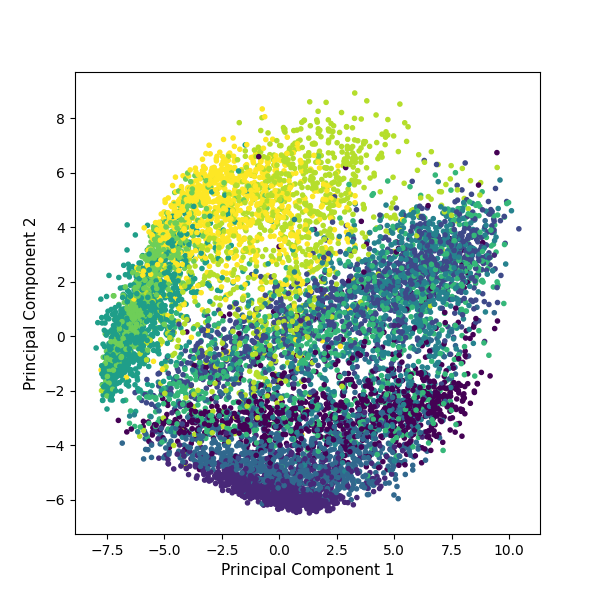
\includegraphics[width=0.35\textheight]{new_images/pca_linear_2comps.png}
			\caption{}
			\label{subfig:pca_linear_2comps}
		\end{subfigure}
		\begin{subfigure}{0.5\textwidth}
			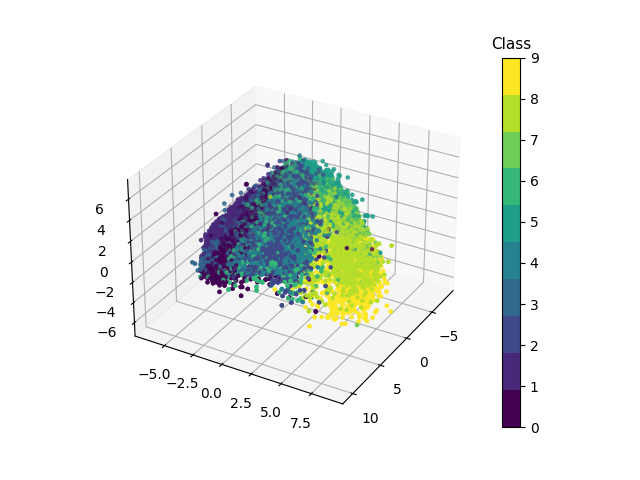
\includegraphics[width=0.35\textheight]{new_images/pca_linear_3comps.png}
			\caption{}
			\label{subfig:lpca_linear_3comps}
		\end{subfigure}
		\caption{First two and three principal components obtained by performing linear PCA, plotted along with true labels}
		\label{fig:pca_linear}
	\end{figure}
	\hfill
	\begin{figure}[h]
		\begin{subfigure}{0.5\textwidth}
			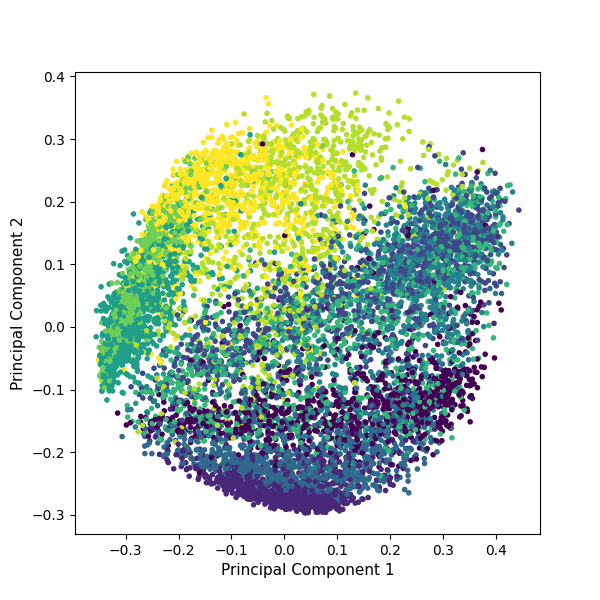
\includegraphics[width=0.35\textheight]{new_images/pca_rbf_2comps.png}
			\caption{}
			\label{subfig:pca_rbf_2comps}
		\end{subfigure}
		\begin{subfigure}{0.5\textwidth}
			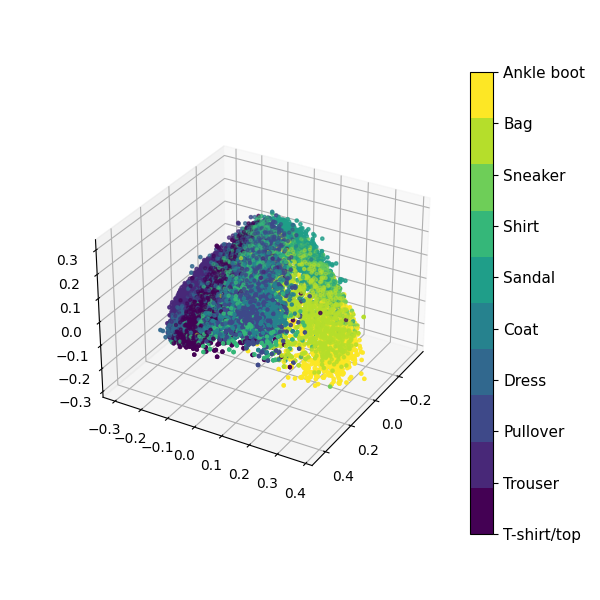
\includegraphics[width=0.35\textheight]{new_images/pca_rbf_3comps.png}
			\caption{}
			\label{subfig:pca_rbf_3comps}
		\end{subfigure}
		\caption{First two and three principal components obtained by performing kernel PCA with RBF kernel, plotted along with true labels}
		\label{fig:pca_rbf}
	\end{figure}
	\hfill
	\begin{figure}[h]
		\begin{subfigure}{0.5\textwidth}
			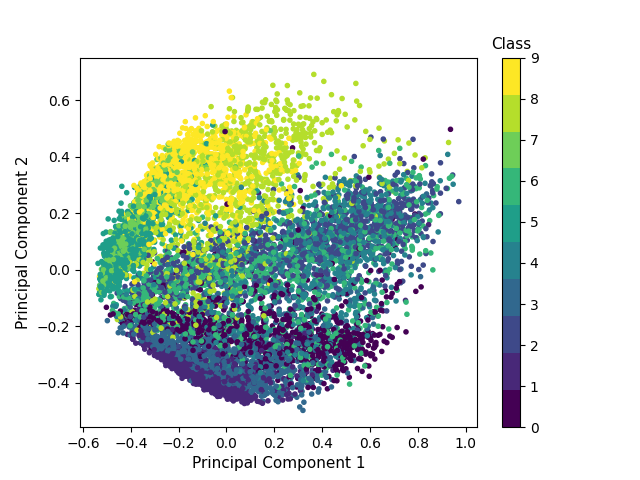
\includegraphics[width=0.35\textheight]{new_images/pca_poly_2comps.png}
			\caption{}
			\label{subfig:pca_poly_2comps}
		\end{subfigure}
		\begin{subfigure}{0.5\textwidth}
			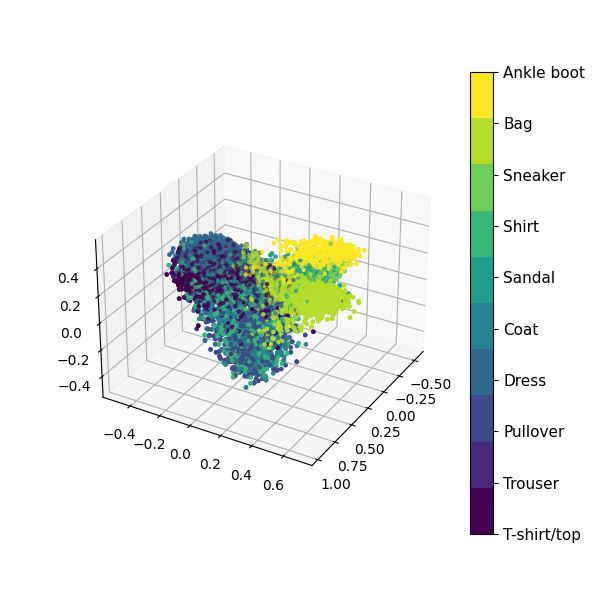
\includegraphics[width=0.35\textheight]{new_images/pca_poly_3comps.png}
			\caption{}
			\label{subfig:pca_poly_3comps}
		\end{subfigure}
		\begin{subfigure}{0.5\textwidth}
			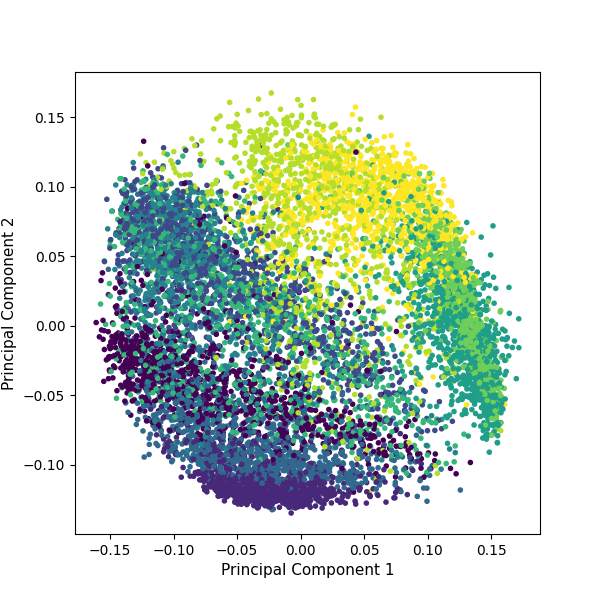
\includegraphics[width=0.35\textheight]{new_images/pca_sigmoid_2comps.png}
			\caption{}
			\label{subfig:pca_sigmoid_2comps}
		\end{subfigure}
		\begin{subfigure}{0.5\textwidth}
			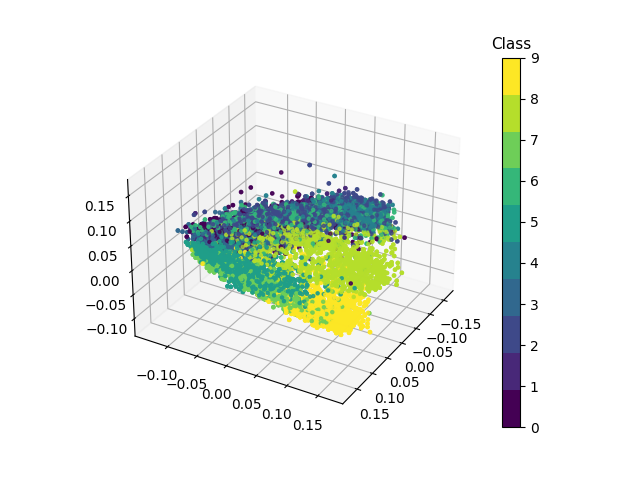
\includegraphics[width=0.35\textheight]{new_images/pca_sigmoid_3comps.png}
			\caption{}
			\label{subfig:pca_sigmoid_3comps}
		\end{subfigure}
		\caption{First two and three principal components obtained by performing kernel PCA with polynomial ((\subref{subfig:pca_poly_2comps}) and (\subref{subfig:pca_poly_3comps})) and sigmoid  ((\subref{subfig:pca_sigmoid_2comps}) and (\subref{subfig:pca_sigmoid_3comps})) kernel, plotted along with true labels.}
		\label{fig:pca_poly_sigmoid}
	\end{figure}
	\hfill
	\begin{figure}[h]
		\centering
		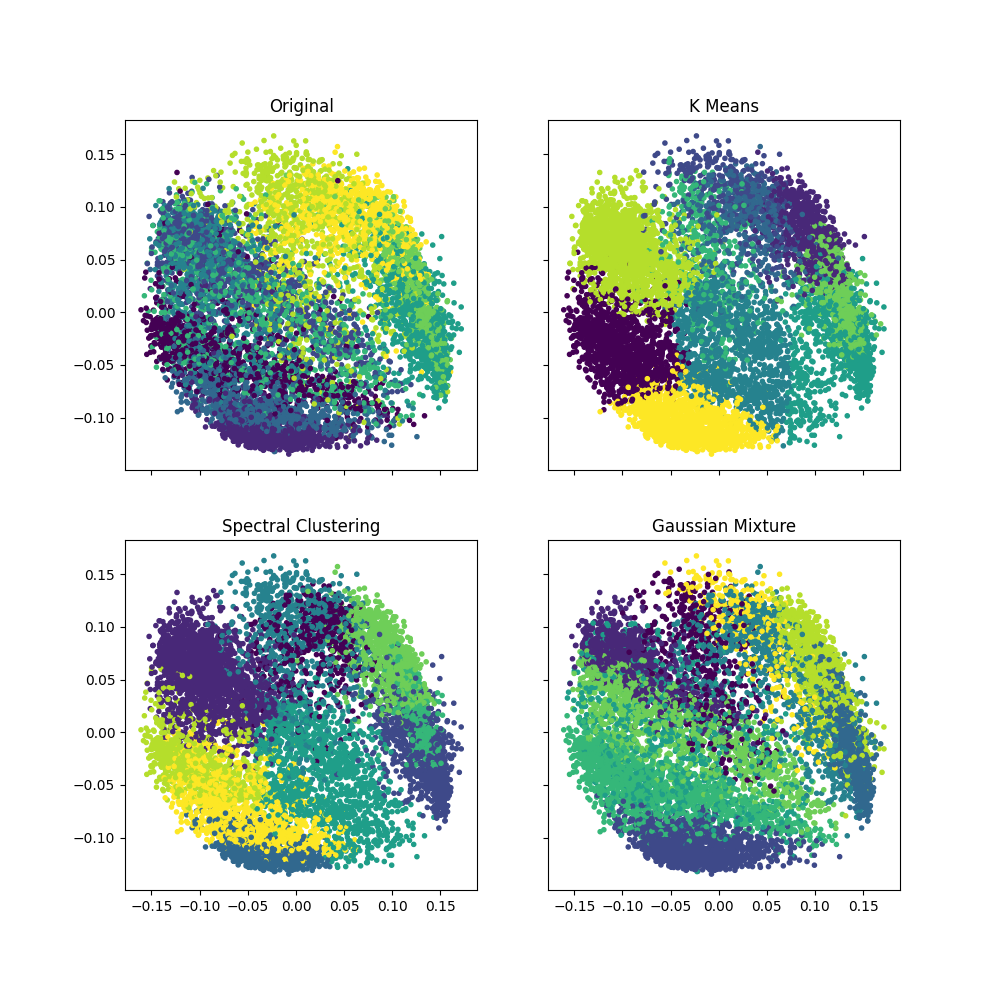
\includegraphics[width = 0.7 \textwidth]{new_images/unsupervised_clustering.png}
		\caption{Unsupervised clustering obtained using K-means clustering, spectral clustering and Gaussian Mixture, confronted with the true labels.}
		\label{fig:unsupervised_clustering}
	\end{figure}
	\hfill
	\begin{figure}[h]
		\centering
		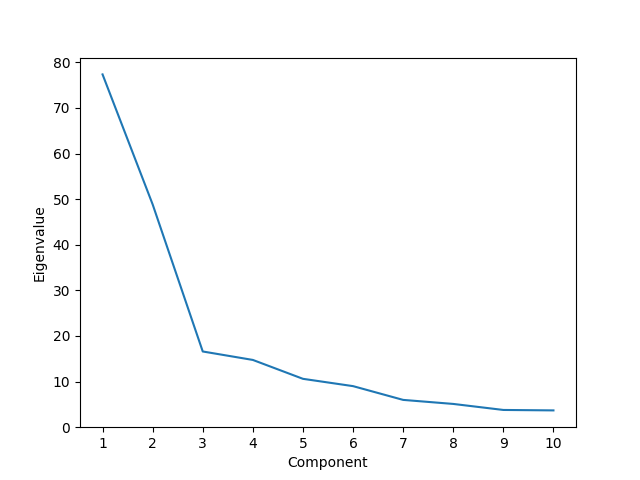
\includegraphics[width = 0.7 \textwidth]{new_images/eigenvalues_sigmoid.png}
		\caption{\protect\parbox{\linewidth}{First 10 eigenvalues obtained by performing kernel PCA with sigmoid kernel.}}
		\label{fig:eigenvalues_sigmoid}
	\end{figure}
	\hfill
	\begin{figure}[h]
		\centering
		\includegraphics[width = 0.7\textwidth]{new_images/ex3-FCNN-comparison-epochs.png}
		\caption{Test accuracy obtained by using a 1-layer and 2-layer fully connected neural network trained for different numbers of epochs}
		\label{fig:ex3_FCNN_epochs}
	\end{figure}
	\hfill
	\begin{figure}[h]
		\centering
		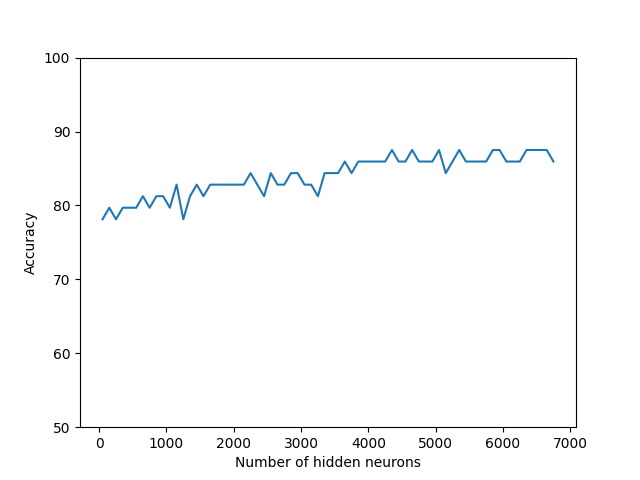
\includegraphics[width = 0.7\textwidth]{new_images/ex3_FCNN2l_accuracy-neurons.png}
		\caption{Test accuracy obtained by using a 2-layer fully connected neural network with different numbers of neurons per hidden layer, trained for 11 epochs}
		\label{fig:ex3_FCNN_neurons}
	\end{figure}
	\hfill
	\begin{figure}[h!]
		\centering
		\includegraphics[width = 0.7\textwidth]
		{new_images/ex3-CNN acc-comparison-epochs.png}
		\caption{Test accuracy obtained by using a 1-layer and 2-layer CNN with 350 neurons per hidden layer, trained for different numbers of epochs}
		\label{fig:ex3_CNN_epochs}
	\end{figure}
	\hfill
	\begin{figure}[h!]
		\centering
		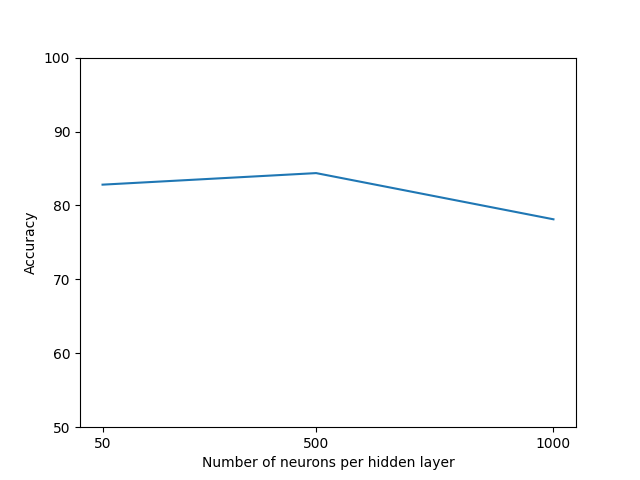
\includegraphics[width = 0.7\textwidth]{new_images/ex3_CNN2l_accuracy-neurons.png}
		\caption{Test accuracy obtained by using a 2-layer convolutional neural network with different numbers of neurons per hidden layer, trained for 3 epochs.}
		\label{fig:ex3_CNN_neurons}
	\end{figure}
	\hfill
	\begin{figure}[h]
		\centering
		\includegraphics[width=0.6\textwidth]{new_images/class4.png}
		\caption{30 samples from predicted class 4.}
		\label{fig:class4}
	\end{figure}
	\hfill
	\begin{figure}[h!]
		\centering
		\includegraphics[width = 0.6\textwidth]{new_images/pipe-acc.png}
		\caption{}
		\label{fig:pipe-acc}
	\end{figure}
	
\end{document}